% (c) 2012-2013 Dimitrios Vrettos - d.vrettos@gmail.com
% (c) 2014 Daniele Zambelli - daniele.zambelli@gmail.com

\chapter{Problemi di I grado in un'incognita}

\section{Un po' di storia e qualche aneddoto}
\label{sec:14_storia}

Sin dall'antichità l'uomo si è
trovato di fronte a difficoltà pratiche, legate alla vita quotidiana
e ha perciò messo a punto strategie per superarle.

Sembra che nell'antico Egitto le periodiche piene del
Nilo abbiano spinto l'uomo a sviluppare la capacità
di tracciare rette parallele, rette perpendicolari, di misurare il
perimetro e l'area di particolari figure geometriche o
viceversa di calcolare le misure dei lati di poligoni di dato perimetro
o data area per poter ridefinire i confini degli appezzamenti di
terreno.

Il \emph{papiro di Rhind}
\footnote{Dal nome dell'inglese A.~H.~Rhind che lo comprò a Luxor nel~1858.}, 
testo egizio scritto in
ieratico, risalente al~1700~\aC, si autodefinisce
``istruzioni per conoscere tutte le cose
oscure'' contiene più di~85 problemi con relativi
metodi di soluzione riguardanti il calcolo della capacità di
recipienti e di magazzini, la ricerca dell'area di
appezzamenti di terreno e altre questioni aritmetiche.

Nel problema~24 del papiro, ad esempio, viene calcolato il mucchio
quando esso ed il suo settimo sono uguali a~19. Mucchio è
l'incognita del problema, indicata con il termine
\emph{aha} il cui segno è
% % (c) 2012 Dimitrios Vrettos - d.vrettos@gmail.com
\begin{hieroglyph}{\leavevmode \loneSign{{\Hsmaller\Aca GD/66/}}}\end{hieroglyph}.

\begin{inaccessibleblock}[Geroglifico]
 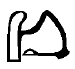
\includegraphics[scale=0.28]{img/giero.png}.
\end{inaccessibleblock}
                                                                  
Noi traduciamo la richiesta nell'equazione~$x+\dfrac{1}{7}x=19$.

Nel~1202 Leonardo Pisano, conosciuto col nome paterno di
`filius Bonacci' o Fibonacci, pubblicò il
\emph{Liber Abaci} in cui, a partire dall'ottavo
capitolo, presenta vari metodi algebrici per la risoluzione di problemi
di matematica applicata, legati alla realtà
dell'epoca, in particolare
all'ambiente commerciale. I nuovi
``algoritmi'' presentati da Fibonacci,
intendevano facilitare la risoluzione dei problemi di calcolo evitando
l'utilizzo dell'abaco. Nel~1223 a
Pisa, l'imperatore Federico~II di Svevia, assistette a
un singolare torneo tra matematici dell'epoca; il
problema proposto era il seguente:

<<Quante coppie di conigli si ottengono in un anno (salvo i
casi di morte) supponendo che ogni coppia dia alla luce
un'altra coppia ogni mese e che le coppie più
giovani siano in grado di riprodursi già al secondo mese di
vita?>>.

Fibonacci vinse la gara dando al quesito una risposta così rapida da
far persino sospettare che il torneo fosse truccato. La soluzione fu
trovata tramite l'individuazione di una particolare
successione di numeri, nota come successione di Fibonacci.

Secondo la leggenda, il grande matematico Carl Fiedrich Gauss già
all'età di tre anni avrebbe corretto un errore di
suo padre nel calcolo delle sue finanze. All'età di
10 anni fu autorizzato a seguire le lezioni di aritmetica di un certo
Buttner. Un giorno, agli studenti particolarmente turbolenti, Buttner
diede come compito di punizione il calcolo della somma dei primi~100
numeri, da~1 a~100. Poco dopo, sorprendendo tutti, il giovanissimo Carl
diede la risposta esatta, ``5050''.
Si era accorto che mettendo in riga tutti i numeri da~1 a~100 e nella
riga sottostante i numeri da~100 a~1, ogni colonna dava come somma~101;
fece dunque il prodotto~$100\times~101$ e divise per~2, ottenendo facilmente il
risultato: Buttner rimase sgomento.

\subsection{Risoluzione dei problemi}

 \epigraph{La risoluzione dei problemi \ldots serve ad acuire
 l'ingegno e a dargli la facoltà di penetrare
 l'intera ragione di tutte le cose.}{{\scshape{R. Descartes}}}


I problemi che possono presentarsi nel corso degli studi o
nell'attività lavorativa sono di diversa natura: di
tipo economico, scientifico, sociale, possono riguardare insiemi
numerici o figure geometriche. La matematica ci può aiutare a
risolvere i problemi quando essi possono essere tradotti in
``forma matematica'', quando cioè
è possibile trascrivere in simboli le relazioni che intercorrono
tra le grandezze del problema.

Analizzeremo problemi di tipo algebrico o geometrico, che potranno
essere formalizzati attraverso equazioni di primo grado in una sola
incognita. Prima di buttarci alla risoluzione del problema, procediamo
a:

\begin{enumeratea}
\item una lettura ``attenta'' del
testo al fine di individuare l'ambiente del problema,
le parole chiave, i dati e le informazioni implicite,
l'obiettivo;
\item la scelta della grandezza incognita e la descrizione
dell'insieme in cui si ricerca il suo valore,
ragionando sull'obiettivo del problema (condizioni sull'incognita);
\item la traduzione in ``forma matematica'' delle relazioni che intercorrono tra 
i
dati e l'obiettivo, cioè l'individuazione dell'equazione risolvente;
\item la risoluzione dell'equazione trovata;
\item il confronto tra la soluzione trovata e le condizioni poste su di essa.
\end{enumeratea}

\begin{problema}
 Un mattone pesa un chilo più mezzo mattone. Quanto pesa un mattone?
\end{problema}

\begin{soluzione}
 La situazione può essere materialmente descritta con una figura.
Togliamo da ogni piatto della bilancia mezzo mattone, la bilancia è
ancora in equilibrio come mostra la figura~2, da ciò possiamo
dedurre che mezzo mattone pesa un chilo. Il mattone intero pesa dunque
due chili.
\begin{center}
 % (c) 2012 Dimitrios Vrettos - d.vrettos@gmail.com
\begin{tikzpicture}[font=\small,x=5mm, y=5mm, scale=.75]

\begin{scope}[fill=black, draw=black]
\filldraw (0,0) rectangle (4,1);
\filldraw[rounded corners=2] (1,1.1)rectangle (3,1.6);
\filldraw (1.8,1.7) rectangle (2.3,8);
\filldraw[rounded corners=2] (1.5,8.1)rectangle (2.6,8.6);
\filldraw (-4,8.7) rectangle (8,9.1);
\filldraw[rounded corners=2] (1.8,8.8)rectangle (2.3,9.8);

\node[name=c1,shape=semicircle,shape border rotate=180, inner sep=3.75mm,draw=black, fill=black] at (-4,3)
{};
\node (a) at (-4,8.7) {};
\draw (a.center)--(c1.arc start);
\draw (a.center)--(c1.arc end);

\node[name=c2,shape=semicircle,shape border rotate=180, inner sep=3.75mm,draw=black, fill=black] at (8,3)
{};
\node (b) at (8,8.7) {};
\draw (b.center)--(c2.arc start);
\draw (b.center)--(c2.arc end);

\filldraw[fill=orange, draw=orange](-5.5,4.02) rectangle (-2.5,5.1);
\filldraw[fill=orange, draw=orange](6.5,4.02) rectangle (8,5.1);
\filldraw[fill=white] (8.3,4) rectangle (9.7,5.1);
\filldraw[fill=white] (8.6,5.1) rectangle (9.4,5.4);
\node () at (9,4.5) {1kg};
\node () at (2,-1) {Figura 1};
\end{scope}

\begin{scope}[fill=black, draw=black, xshift=100mm]
\filldraw (0,0) rectangle (4,1);
\filldraw[rounded corners=2] (1,1.1)rectangle (3,1.6);
\filldraw (1.8,1.7) rectangle (2.3,8);
\filldraw[rounded corners=2] (1.5,8.1)rectangle (2.6,8.6);
\filldraw (-4,8.7) rectangle (8,9.1);
\filldraw[rounded corners=2] (1.8,8.8)rectangle (2.3,9.8);

\node[name=c1,shape=semicircle,shape border rotate=180, inner sep=3.75mm,draw=black, fill=black] at (-4,3)
{};
\node (a) at (-4,8.7) {};
\draw (a.center)--(c1.arc start);
\draw (a.center)--(c1.arc end);

\node[name=c2,shape=semicircle,shape border rotate=180, inner sep=3.75mm,draw=black, fill=black] at (8,3)
{};
\node (b) at (8,8.7) {};
\draw (b.center)--(c2.arc start);
\draw (b.center)--(c2.arc end);

\filldraw[fill=orange, draw=orange](-5,4.02) rectangle (-3,5.1);
\filldraw[fill=white] (7.3,4) rectangle (8.7,5.1);
\filldraw[fill=white] (7.6,5.1) rectangle (8.4,5.4);
\node () at (8,4.5) {1kg};
\node () at (2,-1) {Figura 2};
\end{scope}

\end{tikzpicture}
\end{center}

Risolviamo ora il problema seguendo la procedura sopra suggerita:

\emph{Dati}: peso di un mattone~$=$ peso di mezzo mattone~$+ 1\unit{kg}.$

\emph{Obiettivo}: peso del mattone.

\emph{Procedura risolutiva}:

Come incognita del problema possiamo scegliere il peso del mattone: la
indichiamo con~$p$.
Il valore di~$p$ dovrà essere un numero positivo.
L'equazione risolvente è la traduzione con formalismo
matematico dell'unica relazione contenuta nel testo del
problema:~$p=\frac{1}{2}p+1$.

Risolviamo l'equazione:~$p-\frac{1}{2}p=1\Rightarrow\frac{1}{2}p=1\Rightarrow 
p=2\unit{Kg}.$
La soluzione ottenuta è accettabile; il problema è determinato.
\end{soluzione}

\begin{problema}
 Aggiungendo ad un numero naturale i suoi tre quarti, si ottiene il suo
doppio aumentato di~10. Qual è il numero?
\end{problema}

\begin{soluzione}
L'ambiente del problema è numerico: si cerca un numero
naturale. Indichiamo con~$n$ l'incognita
cerchiamo quindi~$n\in\insN$. La lettura attenta del testo mette
in luce le operazioni che dobbiamo eseguire
sull'incognita e che traduciamo nei dati:

\emph{Dati}:~$n+\dfrac{3}{4}n=2n+10$.

\emph{Obiettivo}:~$n\in\insN$.

\emph{Procedura risolutiva}:

L'equazione risolvente è già indicata nei dati~$n+\dfrac{3}{4}n=2n+10$.

Per risolverla moltiplichiamo ambo i membri per~4, otteniamo:
\[4n+3n-8n=40\Rightarrow -n=40\Rightarrow n=-40.\]

La soluzione non è accettabile per le condizioni poste; il problema
non ha soluzione.
\end{soluzione}

\begin{problema}
 Il~1{\textdegree} gennaio~1990 Chiara aveva il doppio
dell'età di Aldo; il~1{\textdegree} gennaio~2000
Chiara aveva vent'anni più di Aldo. Quale sarà
l'età di Chiara il~1{\textdegree} gennaio~2010?
\end{problema}

\begin{soluzione}
Leggendo attentamente il problema notiamo che le incognite sono due:
l'età di Chiara e l'età di Aldo.
Indichiamo perciò con~$a$ l'età di
Chiara al~1990 e con~$p$ quella di Aldo.

Nel~2000 la loro età sarà aumentata di~10 anni. Naturalmente la
soluzione del problema sarà nell'insieme dei numeri
naturali. Scriviamo dati e obiettivo usando il formalismo matematico:

\emph{Dati}: nel~1990:~$a=2p$, nel~2000:~$a+10=(p+10)+20$.

\emph{Obiettivo}: L'età di Chiara nel~2010.

\emph{Procedura risolutiva}:
Osserviamo che una volta determinata l'età di Chiara
nel~1990, basterà aggiungere a questa~20 per ottenere la soluzione,
pertanto l'età di Chiara nel~2010 è~$a+20$.
Trasformiamo la seconda relazione riportata nei dati sostituendo
l'informazione relativa al~1990,
si ottiene~$2p+10=p+10+20\Rightarrow~2p-p=20\Rightarrow p=20.$
L'età di Aldo nel~1990 era~20, quindi~$a=40$.
Infine, l'età di Chiara nel~2010 è~$40+20=60$.
La soluzione è accettabile; il problema è determinato.
\end{soluzione}

\begin{problema}
 Calcolare l'area di un rettangolo in cui
l'altezza supera $\dfrac{1}{3}$ della base di~8m e il
perimetro è~$\dfrac{20}{7}$ della base stessa.
\end{problema}

\begin{soluzione}
 Il problema è di tipo geometrico e riguarda un rettangolo. Facendo riferimento 
alla figura abbiamo:
\begin{multicols}{2}
 \emph{Dati}:~$AD=\dfrac{1}{3}AB+8$, $2p=\dfrac{20}{7}AB$.

\emph{Obiettivo}: L'$\Area (ABCD).$

\begin{center}
 % (c) 2012 Dimitrios Vrettos - d.vrettos@gmail.com
\begin{tikzpicture}[font=\small,x=8mm, y=3.5mm]

\draw (0,0) rectangle (4,4);

\begin{scope}[left]
\node  at (0,4) {$A$};
\node  at (0,0) {$D$};
\end{scope}

\begin{scope}[right]
\node  at (4,4) {$B$};
\node  at (4,0) {$C$};
\end{scope}
\end{tikzpicture}
\end{center}
\end{multicols}

\emph{Procedura risolutiva}:
$\Area (ABCD)=\text{ misura base }\cdot \text{ misura altezza 
}=\overline{AB}\cdot \overline{AD}$.

Dobbiamo dunque determinare queste due misure. I dati del problema
indicano che la misura dell'altezza dipende da quella
della base; una volta trovata questa misura basta farne un terzo e
aggiungere~8 per avere quella dell'altezza; questo
ragionamento ci fa scegliere come incognita~$\overline{AB}=x$
con~$x$ numero reale positivo.

Traduciamo con formalismo matematico la prima e la seconda relazione
contenuta nei dati:
$\overline{AD}=\dfrac{1}{3}x+8$ e~$2p=\dfrac{20}{7}x$.

Sappiamo che il perimetro di un rettangolo è il doppio della somma
della base con l'altezza. Riscriviamo con linguaggio
matematico anche questa relazione:~$2\cdot 
\left(x+\dfrac{1}{3}x+8\right)=\dfrac{20}{7}x$
che risulta l'equazione risolvente.

Svolgiamo i calcoli e otteniamo~$4x=21\cdot 16\Rightarrow 
x=84\Rightarrow\overline{AB}=84$ e quindi~$\overline{AD}=36$.
Ottenute le misure della base e dell'altezza calcoliamo~$\Area (ABCD)=36\cdot 
84=3024\unit{{m}^{2}}$.
\end{soluzione}

\begin{problema}
In un triangolo rettangolo il perimetro è~$120\unit{cm}$ e un cateto è~$3/5$
dell'ipotenusa. Determinare l'area del
triangolo.
\end{problema}

\begin{soluzione}
 Il problema è di tipo geometrico e riguarda un triangolo rettangolo.
Rappresentiamo il triangolo:

\begin{multicols}{2}

\emph{Dati}:~$C\hat{{A}}B=90\grado$, $2p= 120$, $AC=\dfrac{3}{5}CB$.

\emph{Obiettivo}: L'$\Area (ABC)$.

\begin{center}
 % (c) 2012 Dimitrios Vrettos - d.vrettos@gmail.com
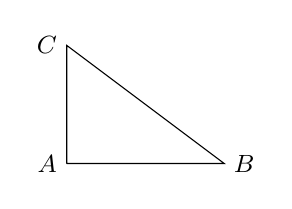
\begin{tikzpicture}[font=\small,x=5mm, y=5mm]

\draw (0,0)-- (4,0)--(0,3)--(0,0);

 \begin{scope}[left]
\node  at (0,3) {$C$};
\node  at (0,0) {$A$};
\end{scope}

\node[right]  at (4,0) {$B$};

\end{tikzpicture}
\end{center}
\end{multicols}

\emph{Procedura risolutiva}:
Dato che $\Area (ABC) =\dfrac{1}{2}\overline{AB}\cdot \overline{AC}$,
dobbiamo calcolare la lunghezza dei cateti.

Il dato $AC=\dfrac{3}{5}CB$ può essere scritto come: $AC=3x \wedge CB=5x$.
L'altro cateto si può calcolare con il teorema di Pitagora:
$AB=\sqrt{(5x)^2-(3x)^2}=\sqrt{25x^2-9x^2}=\sqrt{16x2}=4x$

Il perimetro è: $2p=4x+5x+3x=12x=120$ e da questa equazione ricaviamo 
$x=10$ da cui: $AB=40, BC=50, CA=30$

Da cui si ricava facilmente l'area: 
$\Area=AB \cdot AC \cdot \frac{1}{2} = 40 \cdot 30 \cdot \frac{1}{2} =600$
\end{soluzione}
